% debut d'un fichier latex standard
\documentclass[a4paper,12pt,twoside]{article}

% pour l'inclusion de figures en eps,pdf,jpg
\usepackage{graphicx}
\usepackage{subcaption}
\usepackage{wrapfig}
% quelques symboles mathematiques en plus
\usepackage{amsmath}
% le tout en langue francaise
%\usepackage[french]{babel}
% on peut ecrire directement les caracteres avec l'accent
% a utiliser sur Linux/Windows
\usepackage[utf8]{inputenc}
\usepackage[T1]{fontenc}
% a utiliser sur le Mac
%\usepackage[applemac]{inputenc}
% pour l'inclusion de links dans le document
\usepackage[colorlinks,bookmarks=false,linkcolor=blue,urlcolor=blue]{hyperref}
\usepackage{siunitx}

\paperheight=297mm
\paperwidth=210mm

\setlength{\textheight}{235mm}
\setlength{\topmargin}{-1.2cm} % pour centrer la page verticalement
%\setlength{\footskip}{5mm}
\setlength{\textwidth}{15cm}
\setlength{\oddsidemargin}{0.56cm}
\setlength{\evensidemargin}{0.56cm}

\pagestyle{plain}

% quelques abreviations utiles
\def \be {\begin{equation}}
\def \ee {\end{equation}}
\def \dd  {{\rm d}}

\newcommand{\mail}[1]{{\href{mailto:#1}{#1}}}
\newcommand{\ftplink}[1]{{\href{ftp://#1}{#1}}}
%
% latex SqueletteRapport.tex      % compile la source LaTeX
% xdvi SqueletteRapport.dvi &     % visualise le resultat
% dvips -t a4 -o SqueletteRapport.ps SqueletteRapport % produit un PostScript
% ps2pdf SqueletteRapport.ps      % convertit en pdf

% pdflatex SqueletteRapport.pdf    % compile et produit un pdf

% ======= Le document commence ici ======

\begin{document}
% Le titre, l'auteur et la date
\title{Gravitational systems.\\{\small Apollo 13, atmosphere re-entry and Trojan asteroids \\ Physique Numérique I}\\{\small Rapport 4}}
\date{\today}
\author{Delphine Martres et Damien Korber\\{\small \mail{delphine.martres@epfl.ch} et \mail{damien.korber@epfl.ch}}}
\maketitle
\tableofcontents % Table des matieres

% Quelques options pour les espacements entre lignes, l'identation
% des nouveaux paragraphes, et l'espacement entre paragraphes
\baselineskip=16pt
\parindent=15pt
\parskip=5pt
\newpage


%%%% ON COMMENCE A ECRIRE D'ICI

\section{Introduction}

\section{"Houston, we've had a problem"}
Apollo 13 is located at a distance $r_0 = \SI{314159}{\kilo\meter}$ from the center of Earth.
Its velocity with respect to earth's frame of reference is $v_0 = \SI{1.2}{\kilo\meter\per\second}$.
Because of a fuel shortage, the norm of speed can not be changed.
However, it is possible to ajust its direction.
To bring back Apollo 13's crew, their trajectory needs to get as close as $h=\SI{10}{\kilo\meter}$ to the surface of earth, the distance where the atmosphere is dense enough to slow the ship and break its orbit.
In this experiment, the Moon will be ignored and the mass of Apollo 13 is neglictable compared to Earth's mass. Then, it will be a 1 body gravitationnal problem.
%TODO : Est-ce qu'il faut mettre là toutes les constantes ? Y'en a plein et je les définis quand on en a besoin...

\subsection{Initial velocity of Apollo 13}
The goal of this section is to find the componants of the velocity of the probs, so that it get close to earth, at \SI{10}{\kilo\meter}.
Two physical laws are considered to solve this problem. %TODO : C'est pas des lois, t'as un autre mot ?
\begin{itemize}
  \item Conservation of mechanical energy
  \item Conservation of angular momentum
\end{itemize}

\subsubsection{Conservation of mechanical energy}
The mechanical energy of the probe at any moment is given by equation \eqref{eq:1a-em-apollo13}.
\begin{equation}
  E_m = \frac{1}{2}mv^2 - G\frac{mM}{r}
  \label{eq:1a-em-apollo13}
\end{equation}
where $m=\SI{5809}{\kilo\gram}$ is the mass of the probe, $M=\SI{5.972d24}{\kilo\gram}$ is the mass of earth, $G=\SI{6.674d-11}{\cubic\meter\per\kilo\gram\per\square\second}$ is the gravitational constant, $v$ is the speed of the probe with respect to earth's frame of reference, and $r$ is the distance between the probe and the center of earth.\\

By conservation of mechanical energy, two moments are chosen.
\begin{itemize}
  \item $t=\SI{0}{\s}: E_{m,t_0} = \frac{1}{2}mv_0^2 - G\frac{mM}{r_0}$
  \item $t=t_{end}: E_{m,t_{end}} = \frac{1}{2}mv_{end}^2 - G\frac{mM}{h + R_t}$
\end{itemize}
where $v_0 = \SI{1.2}{\kilo\meter\per\second}$ is the initial velocity of Apollo 13, $r_0 = \SI{314159}{\kilo\meter}$ is the initial distance between Apollo 13 and the center of earth.
Thus, solving $E_{m,t_0} = E_{m,t_{end}}$, the velocity of the probe when it is at a distance $h=\SI{10}{\kilo\meter}$ of earth can be found, and is given by equation \eqref{eq:1a-vitesse-finale}.

\begin{equation}
  v_{end} = \sqrt{v_0^2 + 2GM\left(\frac{1}{h + R_t} - \frac{1}{r_0}\right)}
  \label{eq:1a-vitesse-finale}
\end{equation}

\subsubsection{Conservation of angular momentum}


\subsubsection{Maximum velocity of the probe}
The maximum velocity of the probe on this given situation is given by equation \eqref{eq:1a-vitesse-finale}.
This affirmations comes from the fact that, as the gravitational force is the only one considered, the maximum velocity is given by the moment where the distance is minimal, which is $h_{min}$ in this situation.
Thus, after some computation, the maximum velocity reached by Apollo 13 is given by equation \eqref{eq:1a-vitesse-max}.

\begin{equation}
  v_{max} = \SI{11121.52}{\meter\per\second} %TODO : Donnée à verifier, elle n'est peut-être pas à jour. (calculs.nb)
  \label{eq:1a-vitesse-max}
\end{equation}




\subsection{Numerical analysis with a non-adaptative time step}
In this section, the simulation of the previous simulation will be computed numerically, using the numerical method: Runge-Kutta of order 4 (RK4).

\subsubsection{Trajectory}\label{sec:1b_traj}
The trajectory of Apollo 13 and earth are represented in figure \ref{fig:1b_traj}.
In this figure, earth is considered circular and is drawn at the right scale.
The green cross represents the initial position of Apollo 13, and the green points are its trajectory.
On this figure, the probe seems to come close to Earth, but as drag is not considered, it is not slowed down.
This implicates that the probe gain speed from coming closer to Earth, and then, it continues its path.

\begin{figure}[h]
  \centering
  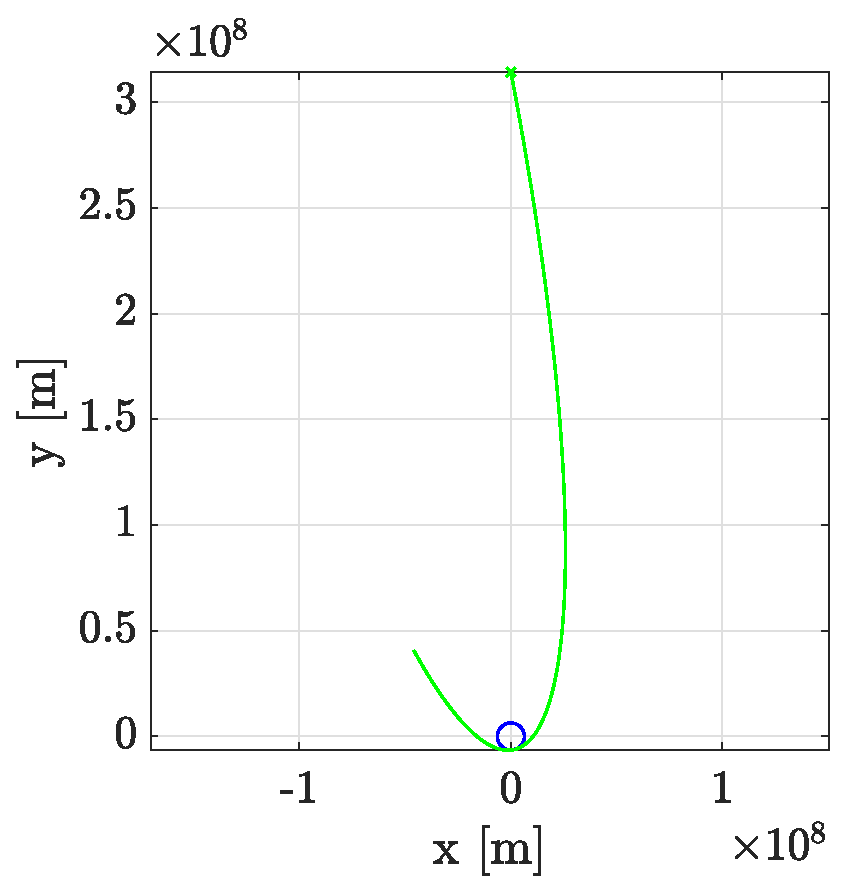
\includegraphics[width=0.5\textwidth]{graphs/ex1b_traj.eps}
  \caption{Trajectory of Apollo 13 (in green, where the cross is its initial position) with Earth (in blue) at the correct scale. The simulation ran with $dt=\SI{50}{\s}$ over \SI{172800}{\s}, and \num{3457} steps where computed.}
  \label{fig:1b_traj}
\end{figure}

\subsubsection{Convergence studies: $h_{min}$ and $v_{max}$}
To study the convergence of RK4, the minimal distance between Earth's surface and Apollo 13, and the maximal speed of Apollo 13 will be studied.
The convergence studies are represented in figure \ref{fig:1b_conv}.

\begin{figure}[h]
  \centering
  \begin{subfigure}[t]{0.45\textwidth}
    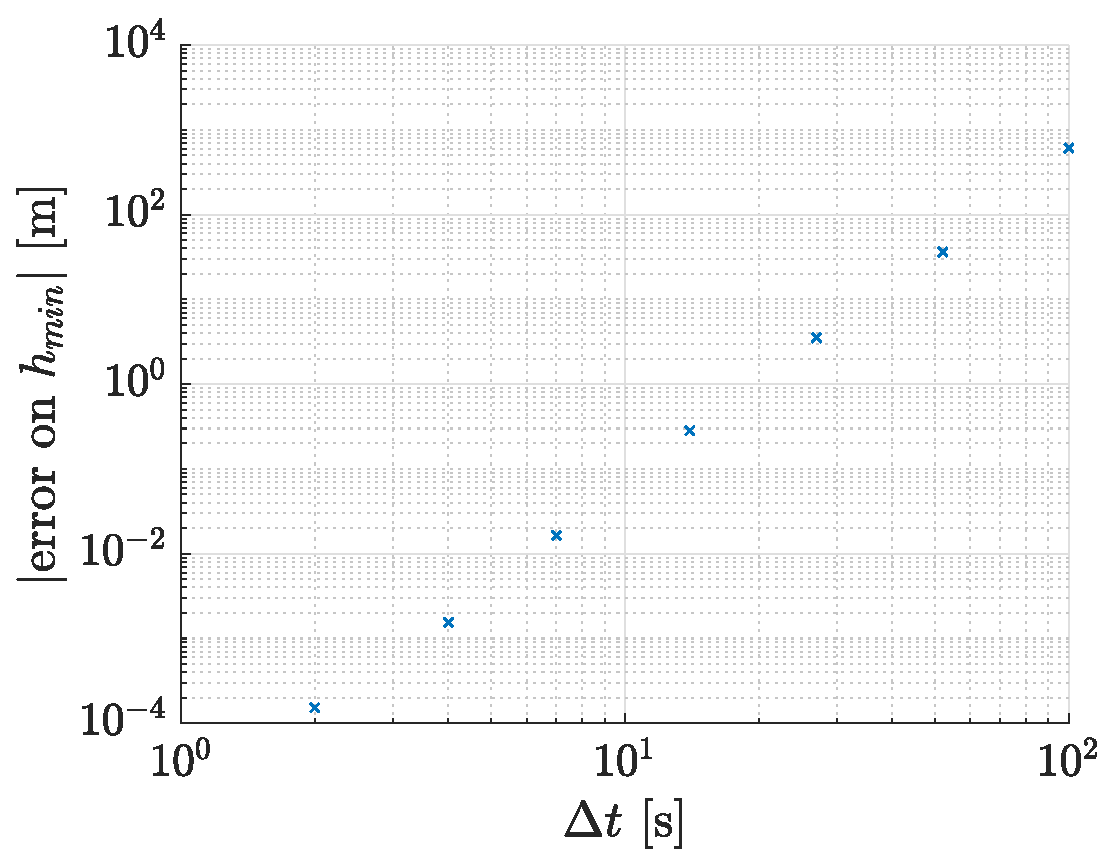
\includegraphics[width=\textwidth]{graphs/ex1b_conv_h.eps}
    \caption{Convergence study on the minimum distance between Apollo 13 and the earth.}
    \label{fig:1b_conv_hmin}
  \end{subfigure}
  ~
  \begin{subfigure}[t]{0.45\textwidth}
    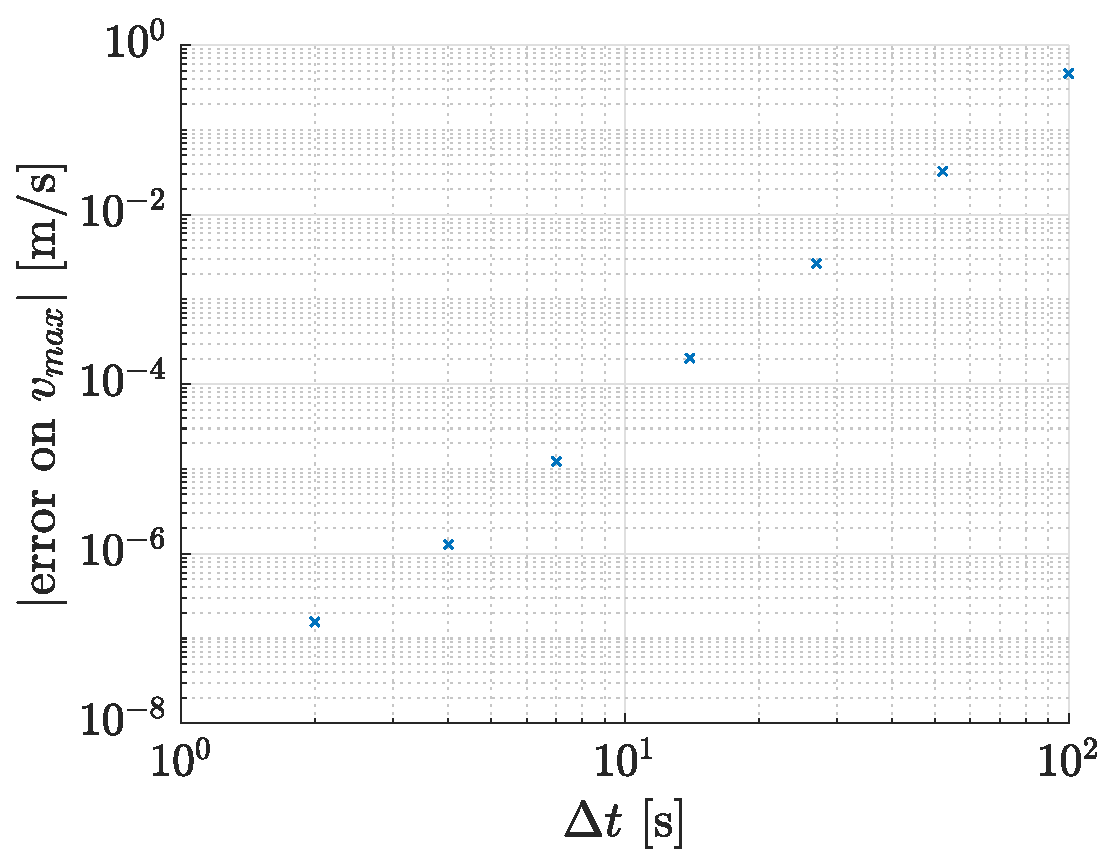
\includegraphics[width=\textwidth]{graphs/ex1b_conv_vel.eps}
    \caption{Convergence study on the maximum velocity of Apollo 13.}
    \label{fig:1b_conv_vmax}
  \end{subfigure}
  \caption{Convergence studies for 10 simulation, with a final time of \SI{172800}{\s} (which is two days).}
  \label{fig:1b_conv}
\end{figure}

The first information to extract from figure \ref{fig:1b_conv} is the fact that both parameters converges.
On figure \ref{fig:1b_conv_hmin}, it can be seen that the error on the minimal distance gets really small, \num{d-3} meters, with respect to the distances considered, which are hundred thousands of kilometers.
The same applies for figure \ref{fig:1b_conv_vmax}, where the error becomes small too.
Thus, RK4 seems to be a good numerical method to get precise results.
The next point is to analyse is the order of convergence, which is given by the slope of the linear regressions.
In both cases, the slope is close to $4$, which is what was expected for a fourth-order numerical method.
Thus, RK4 converges on the expected order for this simulation.

\subsection{Numerical analysis with an adaptative time step}
This time, the same situation is computed numerically, but with an adaptative time step.
It means that, for each steps, the time step is modified, to obtain a particular precision.
It allows to use greater time steps when the evolution is slightly changing, and to use smaller time steps when the evolution is greatly changing.
Thus, it should greatly reduces the number of steps required to do a simulation.

\subsubsection{Trajectory}
The trajectory of the probe is computed with the same conditions than in section \ref{sec:1b_traj}, with the adaptative time step enabled.
Thus, it is possible to compare both results.
The trajectory of the probe is represented in figure \ref{fig:1c_traj}.

\begin{figure}
  \centering
  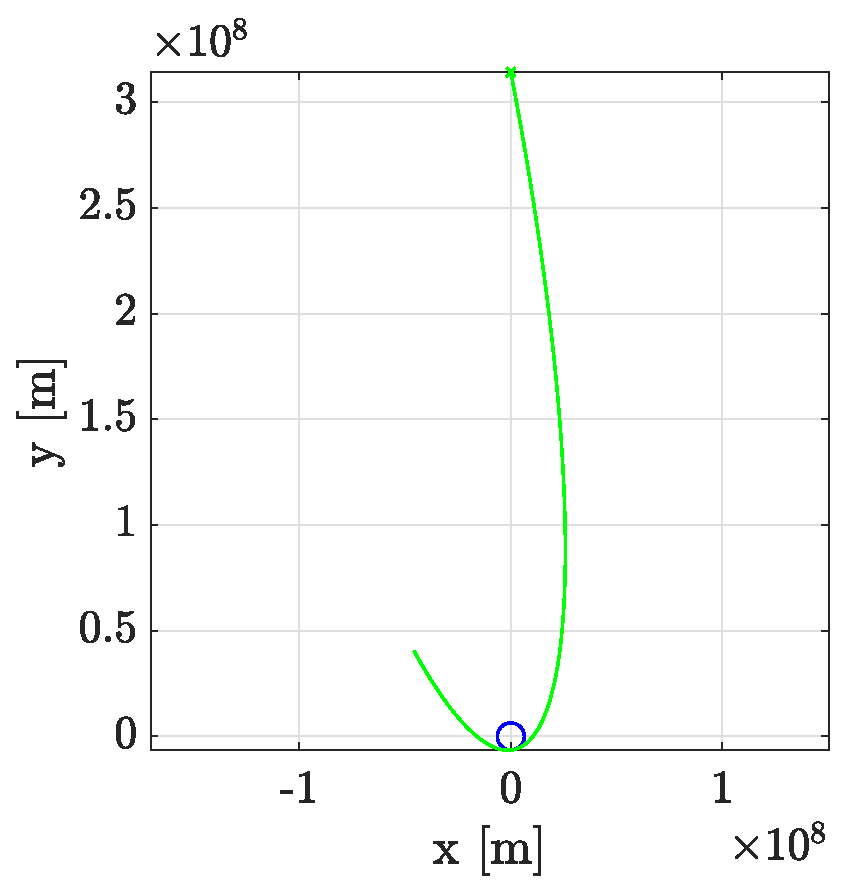
\includegraphics[width=0.5\textwidth]{graphs/ex1c_traj.eps}
  \caption{Trajectory of Apollo 13 (in green, where the cross is its initial position) with Earth (in blue) at the correct scale. The simulation ran with $\epsilon=\SI{d-5}{\m}$ over \SI{172800}{\s}, and \num{1162} steps where computed.}
  \label{fig:1c_traj}
\end{figure}

%TODO: Faire une comparaison des deux trajectoires (1c_traj et 1b_traj), notamment avec les nsteps.
The most important comparison to make between the adaptative and non-adaptative time step's simulations, is the number of steps required to achieve them.
For the non-adaptative time step (fig. \ref{fig:1b_traj}), \num{3457} steps where required to get the solution, but for the adaptative time step (fig. \ref{fig:1c_traj}), \num{1162} steps where required, which is three times less.
On a such simple simulation, the difference between both results is not so significant, as both of them computes quickly.
But on really big simulations (considering millions of steps), this different is not neglectable.
Also, the adaptative time step simulation used a high precision of $\epsilon=\SI{d-5}{\m}$, which may be unnecessary in some sitation.
With a precision of \SI{d-3}{\m}, the solution is already quite good for some problems, and it requires much less time steps to be computed.

\subsubsection{Convergence study on the precision}
The adaptative time step is controlled by a factor, $\epsilon$, which provides the precision that the next step has to reach.
By varying $\epsilon$, the convergence of $h_{min}$ with respect to the number of steps can be studied.
The resulting study is represented in figure \ref{fig:1c_conveps_h}, and figure \ref{fig:1c_conveps_dt} represents the evolution of dt over time for one of the simulation.

\begin{figure}[h]
  \centering
  \begin{subfigure}[t]{0.45\textwidth}
    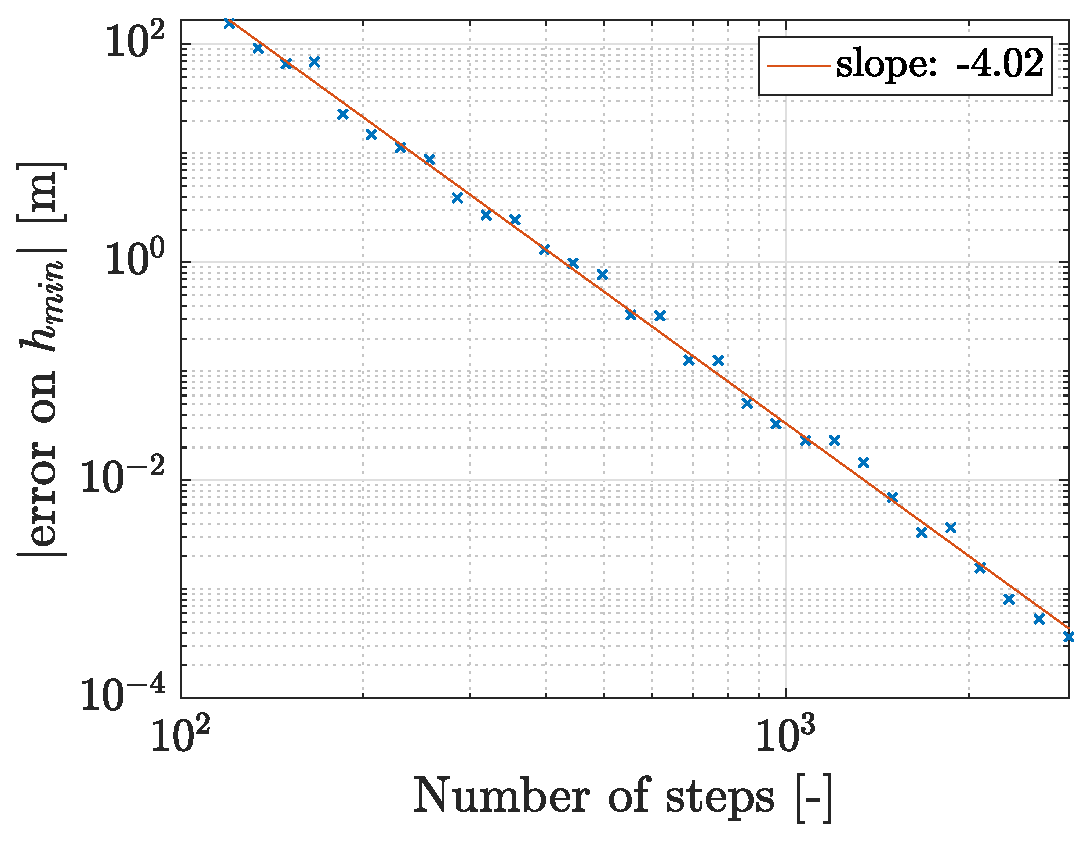
\includegraphics[width=\textwidth]{graphs/ex1c_conveps_h.eps}
    \caption{Convergence study of the minimum distance between Apollo 13 and the Earth.}
    \label{fig:1c_conveps_h}
  \end{subfigure}
  ~
  \begin{subfigure}[t]{0.45\textwidth}
    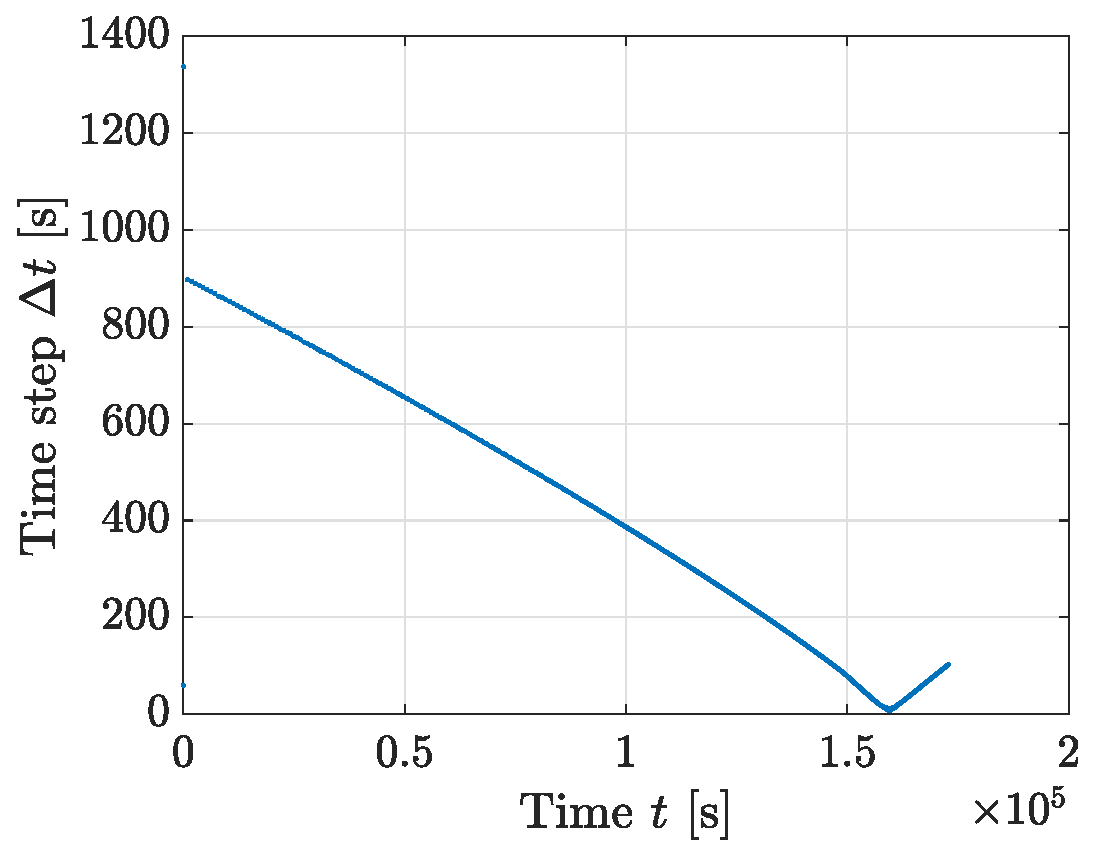
\includegraphics[width=\textwidth]{graphs/ex1c_conveps_dt.eps}
    \caption{Evolution of the time step over time for $\epsilon=\SI{1e-5}{\m}$, and \num{1162} steps were computed.}
    \label{fig:1c_conveps_dt}
  \end{subfigure}
  \caption{Simulations using an adaptative time step. All of the simulations were ran for $\SI{172800}{\s}$.}
  \label{fig:1c_conveps}
\end{figure}

Figure \ref{fig:1c_conveps_h} shows that RK4 converges to the real minimum distance, as the error keeps decreasing linearly (on a log-log plot).
Furthermore, the slope of the linear regression is estimated to $4$, which is the expected order of convergence of RK4.
Figure \ref{fig:1c_conveps_dt} shows the evolution of dt over time, thus shows how the adaptative time steps works.
As the probe approaches Earth, dt keeps decreasing, because of the increasing speed of the probe.
But as soon the probe overtakes Earth, the speed starts decreasing and dt starts increasing.
This result is as expected, and shows that the adaptative time step actually work.

\section{"Houston, we're going to have a real problem"}
In this section, the atmosphere of Earth will be considered.
This allows the probe to return to the ground, hopefully, in safety.

\subsection{Earth re-entry without modifying the initial conditions}
This section studies the possibilities for Apollo 13 to return to Earth, when no modification to the trajectory is applied.\\

First, the trajectory of the probe is represented, to get an idea of the behavious of the probe.
Figure \ref{fig:2a_traj} represents the trajectory of Apollo 13.

\begin{figure}[h]
  \centering
  \begin{subfigure}[t]{0.45\textwidth}
    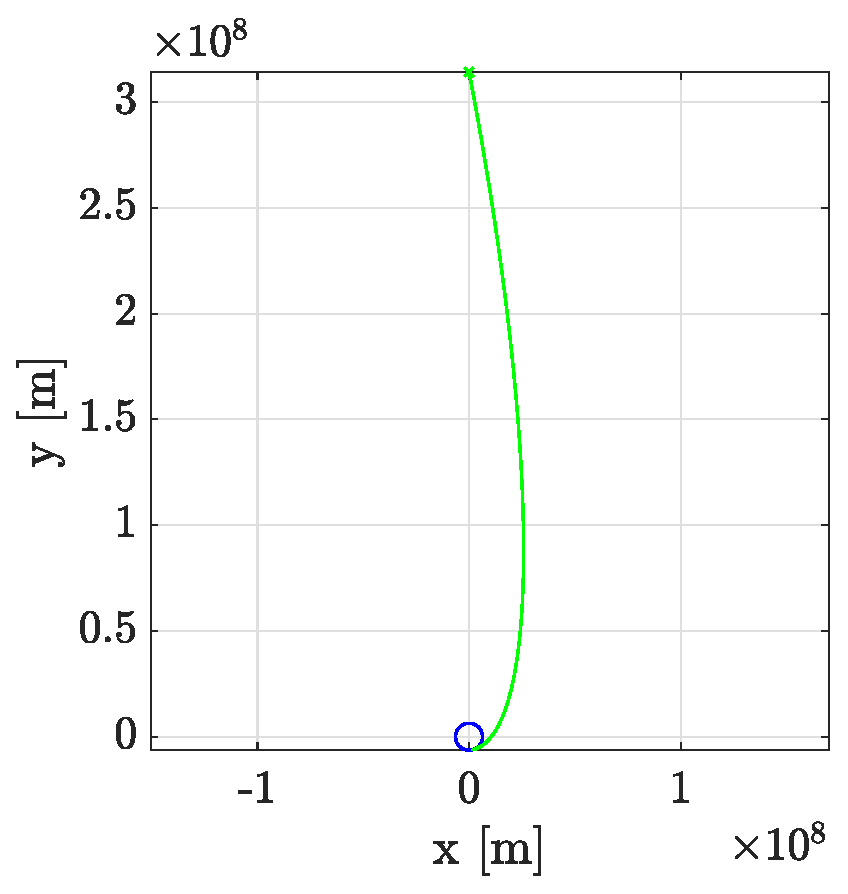
\includegraphics[width=\textwidth]{graphs/ex2a_traj_full.eps}
    \caption{Full trajectory.}
    \label{fig:2a_traj_full}
  \end{subfigure}
  ~
  \begin{subfigure}[t]{0.45\textwidth}
    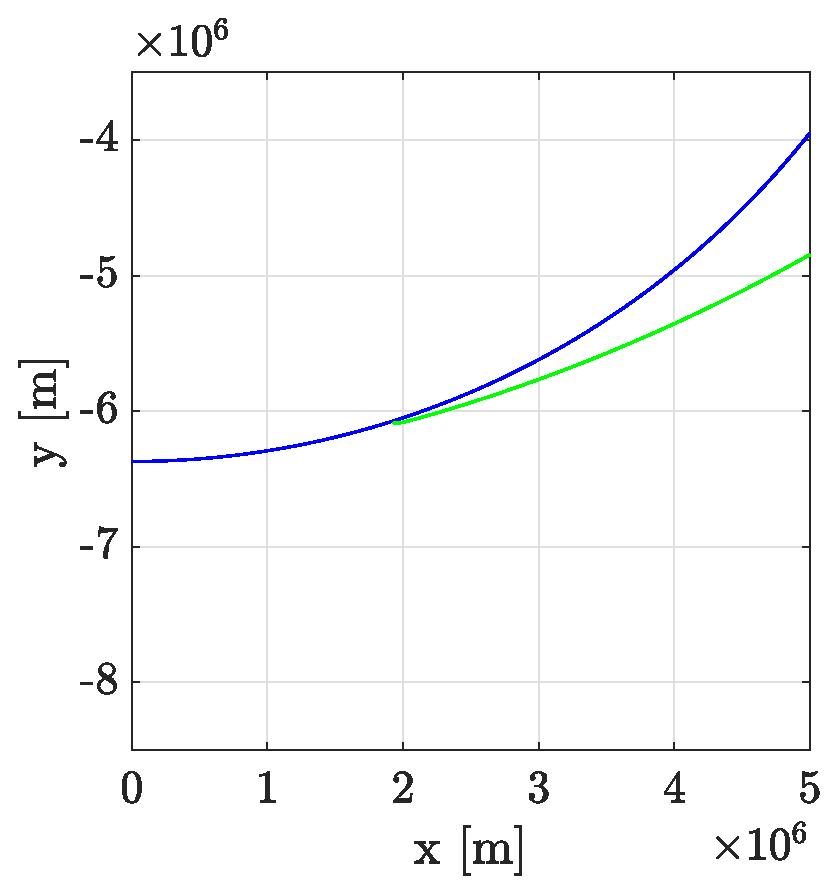
\includegraphics[width=\textwidth]{graphs/ex2a_traj_close.eps}
    \caption{Closer look of figure \ref{fig:2a_traj_full}.}
    \label{fig:fig:2a_traj_close}
  \end{subfigure}
  \caption{Trajectory of Apollo 13 (in green, where the cross is the initial position), and the Earth (in blue) at the right scale. The simulation was supposed to run for \SI{172800}{\s} with an adaptative time step of $\epsilon=\SI{1d-5}{\m}$ but was stopped after \SI{159483}{\s} because Apollo 13 crashed into Earth.}
  \label{fig:2a_traj}
\end{figure}

%TODO: Analyser le graph.

Using these conditions, the maximum acceleration that was experienced by the probe is given by equation \eqref{eq:2a_maxAccel}.

\begin{equation}
  a_\text{max} = \SI{220.53}{\meter\per\square\second} = \num{22.49}\text{ G}
  \label{eq:2a_maxAccel}
\end{equation}

This acceleration is absolutely unbearable for any humain, and probably any other mammals.
To get a comparison, astronauts can experience around $\num{3}\text{ G}$ during a liftoff \cite{nasa:ask_the_crew}, but they are experimented and equipped with g-suits, which reduces the impact of acceleration \cite{wiki:g-suit} on the body.To complete this analysis, a convergence study of the maximum acceleration is given by figure \ref{fig:2a_conv}.\\

\begin{figure}[h]
  \centering
  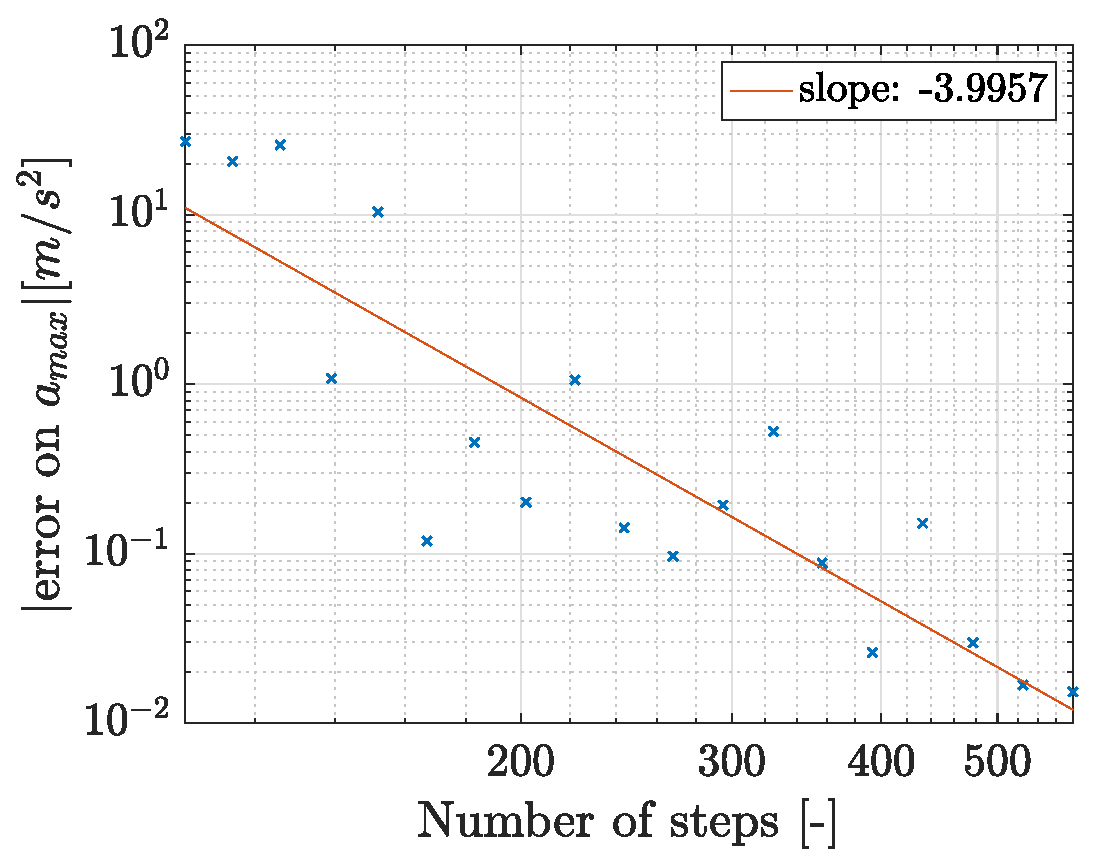
\includegraphics[width=0.5\textwidth]{graphs/ex2a_conv.eps}
  \caption{Convergence study of the error on the maximum acceleration with respect to the number of steps considered. The range of precisions considered is $\epsilon \in [\SI{d-4}{\m}, \SI{1}{\m}]$}
  \label{fig:2a_conv}
\end{figure}

First, it is important to say that the maximum acceleration can not be exactly found, because there is no analytical solution to this problem.
Thus, to consider the error on the maximum acceleration, all the values were compared to the most precise value of the maximum acceleration, which is the one given in equation \eqref{eq:2a_maxAccel}.
On figure \ref{fig:2a_conv}, the main point is the slope of the convergence.
This slope is approximately $4$, which is the expected order of convergence for RK4.
It can also be seen that the error is quite small compared to the considered maximum acceleration, which is given by equation \eqref{eq:2a_maxAccel}.
Thus, RK4 is once again proven to be converging at the right order, and fits the situation well.

The maximum power of the air resistance is given by equation \eqref{eq:2a_maxPower}.

\begin{equation}
  P_{max}(\mathbf{f_\text{drag}}) = \SI{9672252913}{\watt} %TODO: Vérifier les valeurs.
  \label{eq:2a_maxPower}
\end{equation}

% The maximum power described by equation \eqref{eq:2a_maxPower} is big.
%TODO: Un mot sur la puissance peut-être ?

Thus, returning to Earth using the current trajectory is not possible, and another method must be found, which is the topic of next section.


\subsection{Rotating the probe to get the minimal acceleration}
This section will focus on a way to minimize the acceleration underwent by the astronauts in Apollo 13.

The method is quite simple: slightly changing the direction of the initial velocity of the probe.
To achieve this, the initial velocity will be rotated by an angle $\theta$ that will be found in an empirical way.
Note that the probe must land on its first entry in the atmosphere: it should not slow with multiples periods around earth. %TODO : Je trouve cette phrase pas très belle.

Let $\mathbf{v} = \begin{pmatrix} v_1, v_2\end{pmatrix}$ be the initial velocity and $\mathbf{w} = \begin{pmatrix} w_1, w_2\end{pmatrix}$ be the rotated initial velocity.
Both velocities are linked by the rotation matrix, and their relation is given by equation \eqref{eq:v_rotation}.

\begin{equation}
  \begin{pmatrix}
    w_1 \\
    w_2
  \end{pmatrix}
  =
  \begin{pmatrix}
    \cos\theta & -\sin\theta \\
    \sin\theta & \cos\theta
  \end{pmatrix}
  \begin{pmatrix}
    v_1 \\
    v_2 \\
  \end{pmatrix}
  =
  \begin{pmatrix}
    v_1\cos\theta - v_2\sin\theta \\
    v_1\sin\theta + v_2\cos\theta
  \end{pmatrix}
  \label{eq:v_rotation}
\end{equation}

To find the right angle $\theta$ minimizing the acceleration, the plot of the maximum acceleration for a given angle, and the trajectory of the probe, will be use.

Denote $i$ the process number, $\phi_0$ an arbitrary angle and $\Theta_0 = 0$ an angle.
First, an arbitrary range of angles are selected: $A_0 = [\Theta_0-\phi_0, \Theta_0+\phi_0]$.
The rotated velocities $\mathbf{w}$ are computed and stored, for $N$ angles contained in $A$.
These velocities are inserted as the initial velocities, and all the simulations are made.
Next, the two plot cited above are created and analysed.
The plot of trajectory gives an idea of the angles to ignore (those where the probe does not land on the period).
Regarding the left angles, the plot of maximum acceleration gives the best angle in this range, the one giving the smallest maximum acceleration. This angle is denoted by $\Theta_1$.
The process is restarted with a new range of angles $A_1 = [\Theta_1 - \phi_1, \Theta_1 + \phi_1]$, where $\phi_1 < \phi_0$.
By looping $k$ times, until the moment where the minimal acceleration only slightly changes over analysis,  one of the best angle is found.
This angle is given by $\theta = \Theta_k$.

To illustate this method, figure \ref{fig:2b_min_a} gives an example of the plots that can be made for one process.

\begin{figure}[h]
  \centering
  \begin{subfigure}[t]{0.45\textwidth}
    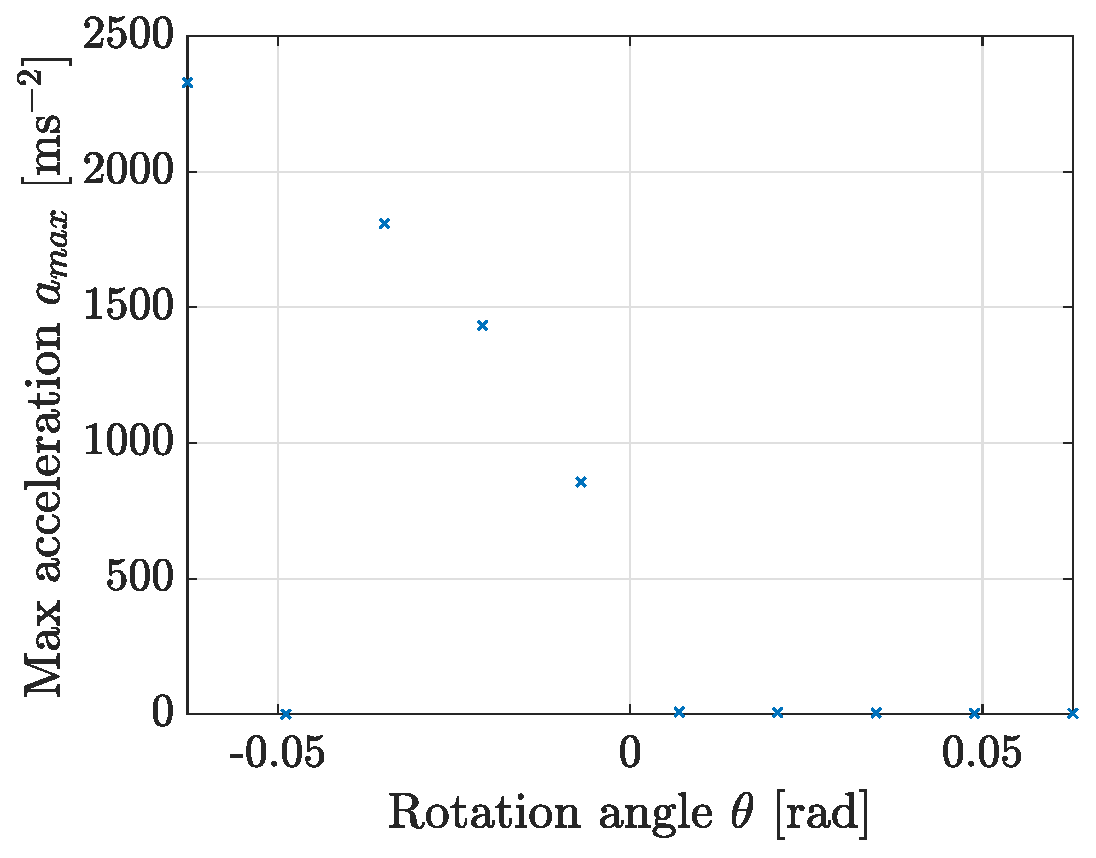
\includegraphics[width=\textwidth]{graphs/ex2b_convacc.eps}
    \caption{Maximum acceleration of all simulations.}
    \label{fig:2b_min_a_traj}
  \end{subfigure}
  ~
  \begin{subfigure}[t]{0.45\textwidth}
    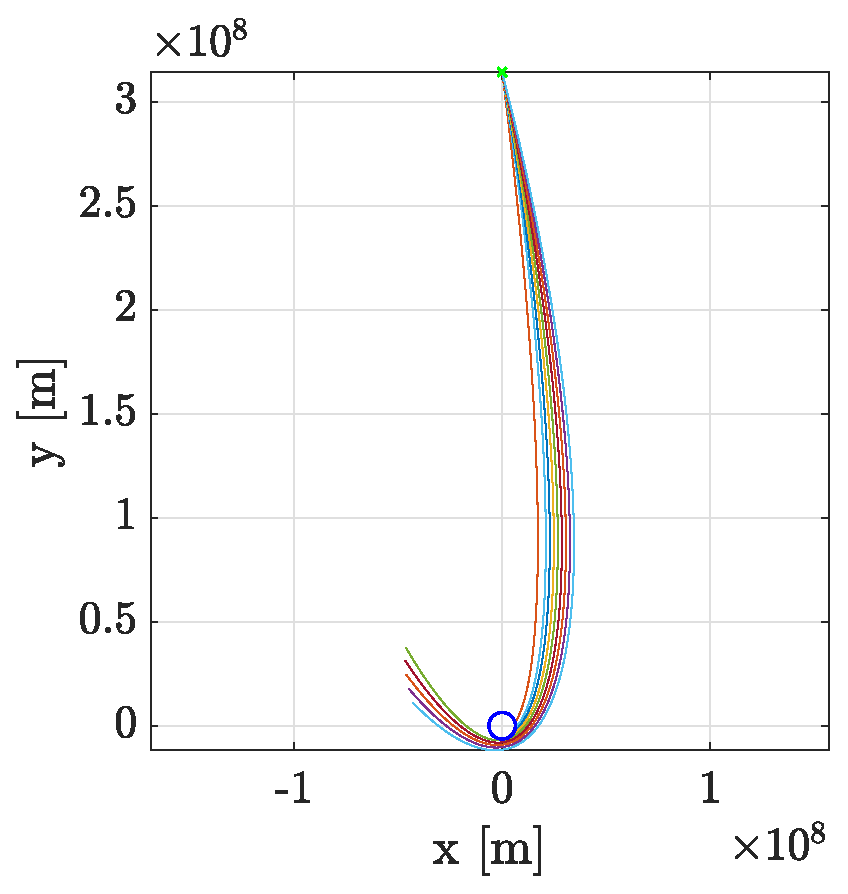
\includegraphics[width=\textwidth]{graphs/ex2b_traj.eps}
    \caption{Trajectories for a given angle. Different colors means different different rotation angles. The legend was removed for readability reasons.}
    \label{fig:2b_min_a_comp}
  \end{subfigure}
  \caption{Study of the trajectory and the maximum acceleration for \num{10} simulations, using an adaptative time step of $\epsilon=1e-4$. The angles of rotations used are contained in the range $[-\frac{\pi}{50}, \frac{\pi}{50}]$.}
  \label{fig:2b_min_a}
\end{figure}

The angle of rotation found using this processes is given by equation \eqref{eq:2b_a_min-angle}.

\begin{equation}
  \theta \approx \SI{5.448956d-4}{\radian} %TODO : Compléter ce résultat.
  \label{eq:2b_a_min_angle}
\end{equation}

The norm of the smallest maximal acceleration, found using angle of equation \eqref{eq:2b_a_min_angle}, is given by equation \eqref{eq:2b_a_min}.

\begin{equation}
  a = \SI{63.29}{\meter\per\square\second} \approx \num{6.45}\text{ G} %TODO : Compléter ce résultat.
  \label{eq:2b_a_min}
\end{equation}

The acceleration in equation \eqref{eq:2b_a_min} is much smaller than the initial acceleration (eq. \eqref{eq:2a_maxAccel}), and is closer to the maximum acceleration astronauts are subjected to.
However, it is still non-neglectable, and astronauts will probably pass out at this moment, but at least, they will land in one piece and have a chance of overcoming this mission.

\section{Two bodies: Earth and Moon}

\section{Three bodies: Earth, Moon and Apollo 13}

\section{Three bodies: Earth, Moon and a third body - Lagrangian points}

\section{Optional}
\subsection{The remaining Lagrangian points}
The section studies the remaining Lagrangian points, which are L1, L2, L3 and L5.

For a 3-body simulation with one neglectable mass, equation \eqref{eq:5b_lagrange_general} gives the general evolution of the third body.
This equation comes from the lessons.

\begin{equation}
  \frac{d^2}{dt^2}
  \begin{pmatrix}
    x' \\
    y'
  \end{pmatrix}
  = -\Omega^2
  \begin{pmatrix}
    \frac{d^3\beta(x' + d\alpha)}{r'^3_{13}} + \frac{d^3\alpha(x' - d\beta)}{r'^3_{23}} - x'\\
    \frac{d^3\beta}{r'^3_{13}}y' + \frac{d^3\alpha}{r'^3_{23}}y' - y'
  \end{pmatrix}
  + 2\Omega\frac{d}{dt}
  \begin{pmatrix}
    y' \\
    -x'
  \end{pmatrix}
  \label{eq:5b_lagrange_general}
\end{equation}

with $\Omega$ the angular momentum of both the Earth (body 1) and the Moon (body 2) in the frame of reference $R'$, $r_{ij}$ the distance between bodies $i$ and $j$, $d$ the distance between the Earth and the Moon, $x'$ ($y'$) the horizontal (vertical) position of the third body, in the frame of reference $R'$, $\alpha = m_2/(m_1 + m_2)$, $\beta = m_1/(m_1 + m_2)$ and $m_i$ the mass of body $i$.\\

In this section, only stationary situations are considered, which means that all derivative are null.
Thus, the equation that will be used is given by equation \eqref{eq:5b_lagrange_stationnaire}.

\begin{equation}
  0
  =
  \begin{pmatrix}
    \frac{d^3\beta(x' + d\alpha)}{r'^3_{13}} + \frac{d^3\alpha(x' - d\beta)}{r'^3_{23}} - x'\\
    \frac{d^3\beta}{r'^3_{13}}y' + \frac{d^3\alpha}{r'^3_{23}}y' - y'
  \end{pmatrix}
  \label{eq:5b_lagrange_stationnaire}
\end{equation}

\subsubsection{Finding L1, L2 and L3}
Points L1, L2 and L3 are particular, because they are all located on the horizontal line, which implicate that $y'=0$.
Thus, for equation \eqref{eq:5b_lagrange_stationnaire}, $r_{ij} = (x'_j - x'_i)\text{sgn}\left(x'_j - x_i\right)$.
To simplify the notation, define $\sigma_i = \text{sgn}\left(x'_j - x'_i\right)$.
The final equation for these point is then given by equation \eqref{eq:5b_lagrange_stationnaire_L123}.

\begin{equation}
  \frac{d^3\beta\left(x' + d\alpha\right)}{\left(x-x_1\right)^3\sigma_1} + \frac{d^3\alpha\left(x' - d\beta\right)}{\left(x-x_2\right)^3\sigma_2} - x' = 0
  \label{eq:5b_lagrange_stationnaire_L123}
\end{equation}

Each of these lagrangian point is determined by $\sigma_i$, at it explains where the third body is with respect to the two others.
Thus:
\begin{itemize}
  \item for L1: $\sigma_1$ = 1, $\sigma_2$ = -1;
  \item for L2: $\sigma_1$ = 1, $\sigma_2$ = 1;
  \item for L3: $\sigma_1$ = -1, $\sigma_2$ = -1.
\end{itemize}

Equation \eqref{eq:5b_lagrange_stationnaire_L123} needs to be solved numerically, as the final polynome is of 7th degree.
Thus, the position of point L1, L2 and L3 are given by:
\begin{itemize}
  \item for L1: $lx_1 = \SI{3.219948720257e8}{\m}$, $ly_1 = \SI{0}{\m}$
  \item for L2: $lx_2 = \SI{4.446515204924e8}{\m}$, $ly_2 = \SI{0}{\m}$
  \item for L3: $lx_3 = \SI{-3.866963974114e8}{\m}$, $ly_3 = \SI{0}{\m}$
\end{itemize}

\subsubsection{Finding L5}
%TODO: À faire

\subsubsection{Stability of all points}
%TODO: À faire


\subsubsection{Representation of Lagrangian points}
To conclude this section, a representation of all the Lagrangian points is drawn in figure \ref{fig:6b_allLPoints}.

\begin{figure}[h]
  \centering
  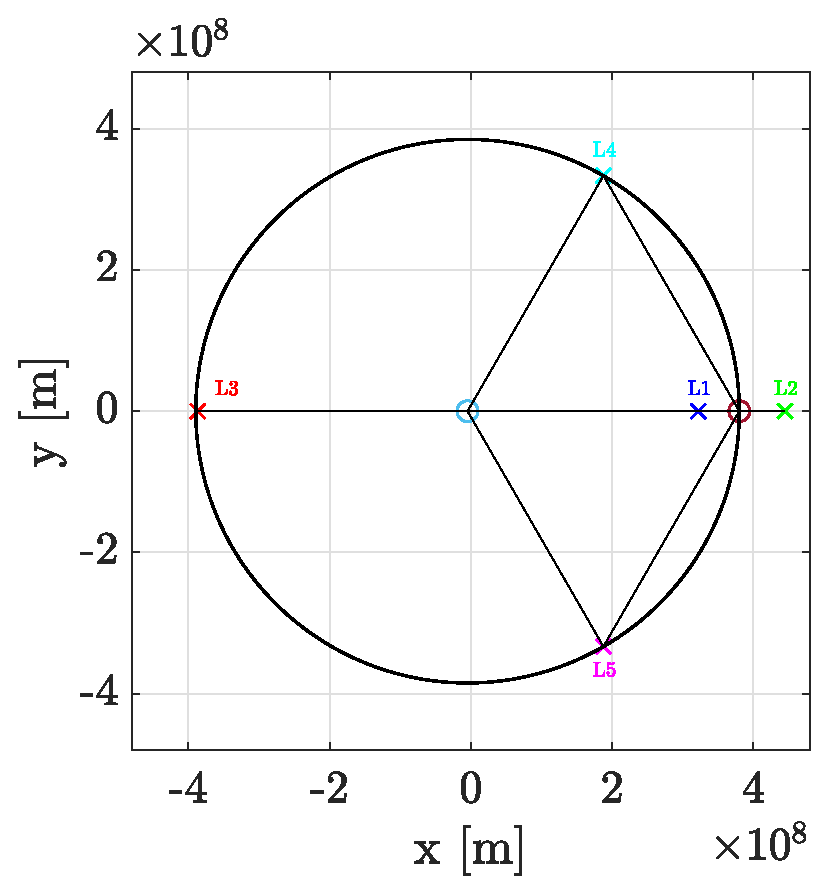
\includegraphics[width=0.5\textwidth]{graphs/ex6b_allLPoints.eps}
  \caption{Representation of all computed Lagrangian points. The origin is the center of gravity between the Earth and the Moon, the blue circle is the Earth (false radius) and the red circle is the Moon (false radius).}
  \label{fig:6b_allLPoints}
\end{figure}



\addcontentsline{toc}{section}{References}
\begin{thebibliography}{99}
  \bibitem{nasa:ask_the_crew} Wakata, K. (2002, April 7). Ask the Crew: STS-92. Retrieved December 14, 2018, from \url{https://spaceflight.nasa.gov/feedback/expert/answer/crew/sts-92/index.html}
  \bibitem{wiki:g-suit} Wikipedia contributors. (2018, December 4). G-suit. In Wikipedia, The Free Encyclopedia. Retrieved 20:59, December 14, 2018, from \url{https://en.wikipedia.org/w/index.php?title=G-suit&oldid=871987759}
\end{thebibliography}
%TODO: Checker l'ordre des références.


\end{document}
